\newpage
\chapter{Cambio de Variables}
Dada una ecuación diferencial de primer orden en forman normal
\begin{equation*}
    \dfrac{dx}{dt} = x' = f(t,x)
\end{equation*}

mediante una función 
\Func{f}{D}{\mathbb{R}}{(t,x)}{f (t,x)}
continua definida en $D\subseteq \mathbb{R}^2$ un conjunto abierto y conexo, nuestro objetivo será, dado un cambio de variable por dos ecuaciones
\begin{equation*}
    \left\{\begin{array}{rl}
        s=\varphi_1(t,x) \\
        y = \varphi_2(t,x)
    \end{array}\right.
\end{equation*}

con 
\Func{\varphi_1,\varphi_2}{D}{\mathbb{R}}{(t,x)}{\varphi_1(t,x), \varphi_2(t,x)}
cambiar tanto la expresión de la ecuación diferencial como el dominio para facilitar la resolución del mismo, mediante una aplicación
\Func{\varphi= (\varphi_1,\varphi_2)}{D}{D_1}{(t,x)}{(s,y)}
con $D_1\subseteq \mathbb{R}^2$ abierto y conexo, que nos lleve a una ecuación diferencial
\begin{equation*}
    \dfrac{dy}{ds} = \hat{f} (s,y)
\end{equation*}

para cierta función
\Func{\hat{f}}{D_1}{\mathbb{R}}{(s,y)}{\hat{f} (s,y)}
Y será de nuestro interés buscar la expresión de dicha $\hat{f}$.\\

Nos preguntamos también por las condiciones que tenemos que exigirle a dicha $\varphi$ para que el cambio de variable sea bueno:
\begin{enumerate}
    \item Que $\varphi$ sea biyectiva, o equivalentemente, que tenga inversa $\psi = \varphi^{-1}$, para poder deshacer el cambio de variable.
    \item Que podamos hacer cálculo diferecial en ambos lados y que podamos transportarlo, es decir, que tanto $\varphi$ como $\psi$ sean de clase $C^1$.
    \item Además, también tendremos que buscar cómo poner $y$ en función de $s$, y exigir hipótesis para que podamos hacerlo.
\end{enumerate}

\begin{definicion}[difeomorfismo]
    Sea $r\in \mathbb{N}$, una aplicación $f:A\rightarrow B$ es un \newline$C^r$-difeomorfismo si $f$ es de clase $C^r(A)$, biyectiva y su inversa $f^{-1}$ es de clase $C^r(B)$.
\end{definicion}
De esta forma, nos interesará que $\varphi$ sea un $C^1$-difeomorfismo, para que se cumplan los dos primeros puntos de la enumeración anterior\footnote{Recordamos que una función de $\mathbb{R}^2$ sea de clase $C^1$ significa que podemos hacer sus derivadas parciales respecto a las dos variables y que ambas son continuas.}.\\

A continuación, realizaremos un razonamiento informal con la finalidad de comprobar qué pasará al realizar el cambio de variable, para luego formalizar el mismo.\\

Volviendo a la situación inicial, nos encontrábamos ante una ecuación de la forma
\begin{equation*}
    \dfrac{dx}{dt} = f(t,x)
\end{equation*}
y nos disponíamos a realizar un cambio de variable
\begin{equation*}
    \left\{\begin{array}{rl}
        s = \varphi_1(t,x) \\
        y = \varphi_2(t,x) 
    \end{array}\right.
\end{equation*}
De esta forma, suponiendo que $x=x(t)$ es solución de la ecuación, tenemos las variables $s$ y $y$ en función de $t$. 
\begin{equation*}
    \left\{\begin{array}{rl}
        s(t) = \varphi_1(t,x(t)) \\
        y(t) = \varphi_2(t,x(t)) 
    \end{array}\right.
\end{equation*}
Suponiendo ahora que podemos expresar $y$ en función de $s$: $y = y(s)$, buscamos calcular:
\begin{equation*}
    \dfrac{dy}{ds} = \dfrac{dy}{dt} \dfrac{dt}{ds}
\end{equation*}
Primero, calculamos:
\begin{equation*}
    \dfrac{dy}{dt} = \dfrac{\partial\varphi_2}{\partial t}(t,x) + \dfrac{\partial\varphi_2}{\partial x}(t,x)x'(t) \AstIg \dfrac{\partial\varphi_2}{\partial t}(t,x) + \dfrac{\partial\varphi_2}{\partial x}(t,x)f(t,x)
\end{equation*}
Donde en $(\ast)$ hemos usado que $x$ era solución de la ecuación diferencial. Posteriormente:
\begin{equation*}
    \dfrac{ds}{dt} = \dfrac{\partial\varphi_1}{\partial t}(t,x) + \dfrac{\partial\varphi_1}{\partial x}(t,x) f(t,x)
\end{equation*}
Así, llegamos a que:
\begin{equation*}
    \dfrac{dy}{ds} = \dfrac{dy}{dt}\dfrac{dt}{ds} = \dfrac{\dfrac{\partial\varphi_2}{\partial t}(t,x) + \dfrac{\partial\varphi_2}{\partial x}(t,x)f(t,x)}{\dfrac{\partial\varphi_1}{\partial t}(t,x) + \dfrac{\partial\varphi_1}{\partial x}(t,x) f(t,x)} 
\end{equation*}
Pero todavía no hemos terminado, ya que ahora tenemos la ecuación diferencial en función de las variables $s$, $y$, $t$ y $x$, por lo que tenemos que terminar de librarnos de las variables $t$ y $x$. Para ello, usamos la función $\psi$, ya que:
\begin{equation*}
    \varphi(t,x) = (s,y) \Longrightarrow \psi(s,y) = (t,x)
\end{equation*}

Sustituyendo:
\begin{equation*}
    \dfrac{dy}{ds} = \dfrac{\dfrac{\partial\varphi_2}{\partial t}(\psi(s,y)) + \dfrac{\partial\varphi_2}{\partial x}(\psi(s,y))f(\psi(s,y))}{\dfrac{\partial\varphi_1}{\partial t}(\psi(s,y)) + \dfrac{\partial\varphi_1}{\partial x}(\psi(s,y)) f(\psi(s,y))}
\end{equation*}
En caso de que el denominador sea distinto de 0, tendremos ya la nueva expresión de la ecuación diferencial, definiendo:
\begin{equation*}
    \hat{f}(s,y) = \dfrac{\dfrac{\partial\varphi_2}{\partial t}(\psi(s,y)) + \dfrac{\partial\varphi_2}{\partial x}(\psi(s,y))f(\psi(s,y))}{\dfrac{\partial\varphi_1}{\partial t}(\psi(s,y)) + \dfrac{\partial\varphi_1}{\partial x}(\psi(s,y)) f(\psi(s,y))}
\end{equation*}
llegamos a que
\begin{equation*}
    \dfrac{dy}{ds} = \hat{f}(s,y)
\end{equation*}

\begin{ejemplo}
    Dada la ecuación diferencial
    \begin{equation*}
        \dfrac{dx}{dt} = \dfrac{\sen(x+t-3)}{{(x-2t+1)}^{2}}
    \end{equation*}
    buscamos aplicarle un cambio de variable.

    La ecuación diferencial así no tiene sentido, pues nos falta darle un dominio de definición: Sea $f:D\subseteq \mathbb{R}^2\rightarrow\mathbb{R}$ una función dada por:
    \begin{equation*}
        f(t,x) = \dfrac{\sen(x+t-3)}{{(x-2t+1)}^{2}}
    \end{equation*}
    Buscamos un conjunto $D$ abierto y conexo que haga que $f$ sea continua.\\

    $f$ es continua en todos los puntos de $\mathbb{R}^2$ salvo en los que se anula su denominador, y esto sucede en la recta
    \begin{equation*}
        x-2t+1= 0
    \end{equation*}
    que divide el plano en dos componentes conexas. Para el dominio de la función $f$, hemos de quedarnos con un semiplano. Elegimos el de la izquierda\footnote{Sin ningún motivo, podría hacerse con el de la derecha.}, por lo que nos quedamos con
    \begin{equation*}
        D = \{(t,x)\in \mathbb{R}^2 \mid x -2t+1>0 \}
    \end{equation*}
    Vamos a aplicarle a esta ecuación diferencial un cambio de variable:
    \begin{equation*}
        \left\{\begin{array}{rll}
            y &= x+t-3 &= \varphi_2(t,x) \\
            s &= x-2t+1 &= \varphi_1(t,x)
        \end{array}\right.
    \end{equation*}
    Primero, veamos que $\varphi = (\varphi_1,\varphi_2)$ es un difeomorfismo de todo el plano en todo el plano:
    \begin{enumerate}
        \item $\varphi$ es biyectiva, ya que se puede despejar de manera única (es un sistema de ecuaciones lineal compatible determinado).
        \item $\varphi$ es de clase $C^1(\mathbb{R}^2)$, ya que sus dos componentes son polinomios.
        \item $\varphi^{-1}$ es de clase $C^1(\mathbb{R}^2)$: ya que al despejar para hallar la expresión de $\varphi^{-1}$, sale que es un polinomio también.
    \end{enumerate}
    Por tanto, $\varphi:\mathbb{R}^2\rightarrow\mathbb{R}^2$ es un $C^1$-difeomorfismo. Sin embargo, nos interesa verlo como un difeomorfismo de $D$. Buscamos su codominio $D_1$ para conseguirlo:\\

    Primero, buscamos qué imagen tiene la recta $x-2t+1=0$, y es la recta $s=0$, que nos divide del plano en dos semiplanos, uno a la izquierda y otro a la derecha. Ahora, la imagen de nuestro conjunto $D$ es el plano de la derecha, ya que tiene que cumplir que:
    \begin{equation*}
        x-2t+1 = s > 0
    \end{equation*}
    En definitiva:
    \begin{equation*}
        D_1 = \{(s,y)\in \mathbb{R}^2 \mid s>0\}
    \end{equation*}
    Además, sabemos que $D_1$ es abierto y conexo.\\

    Ahora, buscamos la fórmula para nuestra aplicación $\hat{f}$. Podríamos usar la fórmula pero vamos a repetir los cálculos:

    \begin{equation*}
        \dfrac{dy}{ds} = \dfrac{dy}{dt}\dfrac{dt}{ds} = \dfrac{\nicefrac{dy}{dt}}{\nicefrac{ds}{dt}}
    \end{equation*}
    Pensando que tanto $y$ como $x$ dependen de $t$:
    \begin{equation*}
        \left.\begin{array}{rl}
            \dfrac{dy}{dt} = x' + 1 \\
            \dfrac{ds}{dt} = x' - 2 
        \end{array}\right\} \Longrightarrow \dfrac{dy}{ds} = \dfrac{x'+1}{x'-2}
    \end{equation*}
    Ahora, usamos que $x$ es solución de la ecuación diferencial, luego se cumplirá que $x'=f(t,x)$:
    \begin{equation*}
        \dfrac{dy}{ds} = \dfrac{x'+1}{x'-2} = \dfrac{\dfrac{\sen(x+t-3)}{{(x-2t+1)}^{2}}+1}{\dfrac{\sen(x+t-3)}{{(x-2t+1)}^{2}}-2}
    \end{equation*}
    A continuación, falta poner la ecuación en función de $(s,y)$. Para ello, componemos con la $\psi$:
    \begin{equation*}
        \dfrac{dy}{ds} = \dfrac{\dfrac{\sen y}{s^2}+1}{\dfrac{\sen y}{s^2}-2} = \dfrac{\sen y+s^2}{\sen y -2s^2} = \hat{f}(s,y)
    \end{equation*}
Finalmente, surge que tenemos que poner la $y$ en función de $s$. La ecuación diferencial no está definida en todo el semiplano: el denominador de la expresión no puede anularse.
Los puntos que cumplan:
\begin{equation*}
    \sen y -2s^2 = 0
\end{equation*}
no pueden entrar en el dominio de la ecuación diferencial.\\

Lo que sucede es que los difeomorfismos transladan curvas en curvas, pero no necesariamente curvas en explícitas a curvas en explícitas, luego puede que una curva que en $D$ se expresaba en explícitas no se pueda expresar en $D_1$ con ecuaciones explícitas, con lo que nos daría una singularidad (en este caso, se anularía dicho denominador). Próximamente, veremos la interpretación gráfica de que esto es lo que realmente sucede.
\end{ejemplo}

Ahora, precedemos a realizar una teoría formal que sustente todas las cuentas realizadas hasta el momento.

\begin{definicion}[Cambio de variable admisible]
    Dada una ecuación diferencial de primer orden en forma normal
    \begin{equation*}
        x'=f(t,x)
    \end{equation*}
    Con $f:D\subseteq \mathbb{R}^2\rightarrow\mathbb{R}$ una función continua con $D$ un conjunto abierto y conexo, un cambio de variable admisible es una transformación:
    \Func{\varphi= (\varphi_1,\varphi_2)}{D}{D_1}{(t,x)}{(s,y)}
    con $D$, $D_1\subseteq \mathbb{R}^2$ abiertos y conexos, $\varphi$ es $C^1$-difeomorfismo, y además cumple la condición de admisibilidad\footnote{Esta última condición nos permite que podamos llevar curvas en explícitas $x=x(t)$ que son solución de la ecuación diferencial en $D$ a curvas en explícitas $y=y(s)$ que son solución de la ecuación diferencial en $D_1$.}:
    \begin{equation}\label{eq:condicion_cambio_admisible}
        \dfrac{\partial\varphi_1}{\partial t}(t,x) + \dfrac{\partial\varphi_1}{\partial x}(t,x)f(t,x) \neq 0 \qquad \forall (t,x) \in D
    \end{equation}
\end{definicion}

\begin{teo}[Cambio de variable para ecuaciones diferenciales]
    Dado una ecuación diferencial de primer orden en forma normal
    \begin{equation}\label{eq:dif_1er_orden_fn}
        x'=f(t,x)
    \end{equation}
    Con $f:D\subseteq \mathbb{R}^2\rightarrow\mathbb{R}$ una función continua con $D$ un conjunto abierto y conexo. Sea $\varphi:D\rightarrow D_1$ un cambio de variable admisible.

    Entonces, la ecuación~\ref{eq:dif_1er_orden_fn} es equivalente\footnote{Quiere decir, que siempre que tengamos una curva en $D$ que sea solución de la ecuación diferencial, podamos ir a $D_1$ aplicando $\varphi$ y tendremos una solución de la ecuación diferencial definida en $D_1$, así como este mismo procedimiento al revés.} a la ecuación
    \begin{equation}\label{eq:dif_1er_orden_fn_cambiada}
        \dfrac{dy}{ds} = \hat{f}(s,y)
    \end{equation}

    donde
    \begin{equation*}
        \hat{f}(s,y) = \dfrac{\dfrac{\partial\varphi_2}{\partial t}(\psi(s,y))+\dfrac{\partial\varphi_2}{\partial x}(\psi(s,y))f(\psi(s,y))}{\dfrac{\partial\varphi_1}{\partial t}(\psi(s,y)) + \dfrac{\partial\varphi_1}{\partial x}(\psi(s,y))f(\psi(s,y))} \qquad \forall (s,y)\in D_1
    \end{equation*}

\begin{proof}
    Supongamos que $x=x(t)$ es solución de la ecuación~\ref{eq:dif_1er_orden_fn} definida en un intervalo abierto $I\subseteq \mathbb{R}$, y queremos realizar el cambio
    \begin{equation*}
        \left\{\begin{array}{rl}
            s = \varphi_1(t,x(t)) \\
            y = \varphi_2(t,x(t))
        \end{array}\right.
    \end{equation*}
    Defino
    \Func{S}{I}{\mathbb{R}}{t}{\varphi_1 (t,x (t))}
    que es derivable por la regla de la cadena, con derivada distinta de 0:
    \begin{equation*}
        S'(t) = \dfrac{\partial\varphi_1}{\partial t}(t,x) + \dfrac{\partial\varphi_1}{\partial x}(t,x)x'(t) = \dfrac{\partial\varphi_1}{\partial t}(t,x) + \dfrac{\partial\varphi_1}{\partial x}(t,x)f(t,x) \neq 0 \qquad \forall t\in I
    \end{equation*}
    ya que el cambio era admisible. Defino $J=S(I)$ intervalo abierto, y podemos ahora aplicar el Teorema de la función inversa sobre $S$, obteniendo una función
    \Func{T}{J}{I}{t}{T (s)}
    de forma que cumpla
    \begin{gather*}
        T(S(t)) = t \quad \forall t\in I \\
        S(T(s)) = s \quad s\in J
    \end{gather*}
    Teníamos $s$ en función de $t$ y ahora hemos puesto $t$ en función de $s$ utilizando la primera ecuación del cambio de variable. Ahora, podemos definir (usando la segunda ecuación del cambio) la siguiente función, para expresar $y$ en función de $s$, gracias a que hemos expresado $t$ en función de $s$:
    \Func{y}{J}{\mathbb{R}}{s}{\varphi_2 (T (s), x (T (s)))}
    Nos falta derivar $y$ respecto a $s$ para comprobar que sea solución de la ecuación diferencial~\ref{eq:dif_1er_orden_fn_cambiada}:
    \begin{align*}
        y'(s) &= \dfrac{\partial\varphi_2}{\partial t}(T(s),x(T(s)))\cdot T'(s) + \dfrac{\partial \varphi_2}{\partial x}(T(s),x(T(s)))\cdot x'(T(s))\cdot T'(s) \\
              &= T'(s) \left(\dfrac{\partial\varphi_2}{\partial t}(T(s),x(T(s)))+ \dfrac{\partial \varphi_2}{\partial x}(T(s),x(T(s)))\cdot x'(T(s))\right) \\
              &= T'(s) \left(\dfrac{\partial\varphi_2}{\partial t}(T(s),x(T(s)))+ \dfrac{\partial \varphi_2}{\partial x}(T(s),x(T(s)))\cdot f(T(s),x(T(s)))\right) \\
    \end{align*}
    Ahora, usamos que $\varphi$ tiene de inversa a $\psi$, para así poder expresar
    \begin{equation*}
        \psi(s,y(s)) = (T(s), x(T(s)))
    \end{equation*}

    y eliminar $t$ y $x$ de la expresión, dejándolo todo en función de $s$ e $y$:
    \begin{equation*}
        y'(s) = T'(s) \left(\dfrac{\partial\varphi_2}{\partial t}(\psi(s,y(s)))+ \dfrac{\partial \varphi_2}{\partial x}(\psi(s,y(s)))\cdot f(\psi(s,y(s)))\right)
    \end{equation*}
    Falta ver que $T'(s)$ es el denominador de la expresión~\ref{eq:dif_1er_orden_fn_cambiada}. Para ello, aplicamos la regla de derivación de la función inversa:
    \begin{equation*}
        T'(s) = \dfrac{1}{S'(T(s))} =  \dfrac{1}{\dfrac{\partial\varphi_1}{\partial t}(T(s),x(T(s))) + \dfrac{\partial\varphi_1}{\partial x}(T(s),x(T(s)))f(T(s),x(T(s)))} 
    \end{equation*}
    Ahora, volvemos a usar que
    \begin{equation*}
        \psi(s,y(s)) = (T(s), x(T(s)))
    \end{equation*}

    para obtener
    \begin{equation*}
        T'(s) = \dfrac{1}{S'(T(s))} =  \dfrac{1}{\dfrac{\partial\varphi_1}{\partial t}(\psi(s,y(s))) + \dfrac{\partial\varphi_1}{\partial x}(\psi(s,y(s)))f(\psi(s,y(s)))} 
    \end{equation*}
    Finalmente, falta ver que si tenemos una solución en $D_1$, volvemos a tener una solución en $D$. Bastaría aplicar el mismo proceso pero al revés. Sin embargo, debemos comprobar que si $\varphi$ es admisible para la ecuación~\ref{eq:dif_1er_orden_fn}, entonces $\psi$ lo es para la ecuación~\ref{eq:dif_1er_orden_fn_cambiada}.

    Faltaría comprobar la expresión análoga a~\ref{eq:condicion_cambio_admisible} para $\psi$, esto es:
    % // TODO: Hacer:
    % Demostrar que si \varphi es admisible para x' entonces \psi es admisible para y', es decir, que la condición de \neq 0 se mantiene:
    \begin{equation*}
        \dfrac{\partial\psi_1}{\partial s}(s,y) + \dfrac{\partial\psi_1}{\partial y}(s,y)\hat{f}(s,y) \neq 0 \qquad \forall (s,y) \in  D_1
    \end{equation*}

    Usando que:
    \begin{equation*}
        \varphi'(\psi(s,y))\psi'(s,y) = Id
    \end{equation*}
    % Demostrado esto, veríamos que la condición es equivalente.
\end{proof}
\end{teo}

\section{Ecuaciones sencillas}
Nos falta ahora aprender estrategias para buscar el cambio de variable adecuado en cada caso. Para ello, aprenderemos primero a resolver las ecuaciones diferenciales más sencillas para así cuando se nos presente una más complicada, aplicar un cambio de variable para obtener una ecuación sencilla que sí sepamos resolver.

\subsection{Cálculo de primitivas}
Buscamos resolver ecuaciones diferenciales sencillas. Las ecuaciones diferenciales más sencillas que podemos encontrarnos son el cálculo de primitivas, es decir, cuando la derivada de $x$ sólo está en función de $t$.\\

Pensamos en la ecuación diferencial:
\begin{equation}\label{eq:dif_primitiva}
    x' = p(t)
\end{equation}
con $p:I\subseteq \mathbb{R}\rightarrow\mathbb{R}$ continua, el dominio de la ecuación diferencial es $D = I\times \mathbb{R}\subseteq \mathbb{R}^2$. Sabemos que dicha ecuación diferencial tiene solución, gracias al Teorema Fundamental del Cálculo:

\begin{teo}[Teorema Fundamental del Cálculo]
    Sea $p:I\rightarrow\mathbb{R}$ una funcion continua, fijado $t_0\in I$, entonces
    \begin{equation*}
        P(t) = \int_{t_0}^{t} p(s)~ds 
    \end{equation*}
    es una función de clase $C^1(I)$ que cumple $P'(t) = p(t)$.
\end{teo}
Por tanto, fijado $t_0 \in I$, las soluciones de la ecuación diferencial~\ref{eq:dif_primitiva} son de la forma:
\begin{equation*}
    x(t) = k + \int_{t_0}^{t} p(s)~ds  \qquad k\in \mathbb{R}
\end{equation*}

Tenemos una primera clase de ecuaciones diferenciales que sabemos resolver, al menos a nivel teórico, ya que hay integrales que no pueden calcularse.

\subsection{Ecuaciones de variables separadas}
Una ecuación de variables separadas es una ecuación de la forma
\begin{equation*}
    x' = p(t) q(x)
\end{equation*}
con funciones
\Func{p}{I}{\mathbb{R}}{t}{p(t)}
\Func{q}{J}{\mathbb{R}}{x}{q(x)}
continuas con $I,J\subseteq \mathbb{R}$ intervalos abiertos. De esta forma, estamos manejando la ecuación diferencial
\begin{equation*}
    x' = f(t,x)
\end{equation*}

con
\Func{f}{D=I\times J}{\mathbb{R}}{(t,x)}{p (t) q (x)}

\begin{observacion}
Notemos que el cálculo de primitivas es caso particular de las ecuaciones de variables separadas, ya que tomando $q(x) = 1$ $\forall x\in \mathbb{R}$:
\begin{equation*}
    p(t)q(x) = p(t) \qquad \forall t\in I
\end{equation*}
\end{observacion}
Para su resolución, comenzaremos primero con unos cálculos informales que luego formalizaremos. Dada la ecuación:
\begin{equation*}
    \dfrac{dx}{dt} = p(t)q(x)
\end{equation*}
Primero, buscaremos los valores $a\in J$ que hagan que $q(a) = 0$. En dicho caso, podemos definir la función
\begin{equation*}
    x(t) = a \quad t\in I
\end{equation*}
que es solución de la ecuación diferencial. \\

Una vez localizados todos los ceros de la ecuación, tendremos ya todas las soluciones constantes localizadas. Ahora, haremos separación de variable, que precisamente busca las soluciones que no son constantes. Hacemos la siguiente operación, que por ahora carece de rigor:
\begin{equation*}
    \dfrac{dx}{q(x)} = p(t)~dt
\end{equation*}
Posteriormente, tomaremos primitivas en ambos lados:
\begin{equation*}
    \int\dfrac{dx}{q(x)} = \int p(t)~dt \\
\end{equation*}
Notando por $\Phi$ a una primitiva para $\frac{1}{q}$ y por $P$ a una primitiva de $p$, tendremos que:
\begin{equation*}
    \Phi(x)+c_1 = P(t) + c_2
\end{equation*}
Para ciertas constantes arbitrarias $c_1,c_2\in \mathbb{R}$. Sin embargo, como la diferencia de constantes sigue siendo una constante, podemos escribir simplemente:
\begin{equation*}
    \Phi(x)= P(t) + c
\end{equation*}
Si ahora podemos calcular una inversa de $\Phi$ (en caso de que esta sea biyectiva), podemos deducir que:
\begin{equation*}
    x(t) = \Phi^{-1}(P(t)+c)
\end{equation*}

\begin{ejemplo}
    En este ejemplo, mostraremos que el procedimiento anterior parece funcionar ante las ecuaciones diferenciales de variables separadas, pese a carecer de sentido aparente. Para ello, trataremos de resolver la ecuación
    \begin{equation*}
        x' = e^{t+x}
    \end{equation*}
    con dominio $D=\mathbb{R}^2$, que es una ecuación en variables separadas, ya que:
    \begin{equation*}
        x' = e^{t+x} = e^t e^x
    \end{equation*}
    En este caso, no encontramos soluciones constantes, ya que $e^x>0$ $\forall x\in \mathbb{R}$. Resolvámosla con la receta que acabamos de aprender:
    \begin{gather*}
        \dfrac{dx}{dt} = e^t e^x \\
        e^{-x}~dx = e^t~dt \\
        \int e^{-x}~dx = \int e^t~dt \\
        -e^{-x} = e^t + c
    \end{gather*}
    La última igualdad nos da la función $x$ de manera implícita, buscamos ahora la forma de dar la función $x$ de forma explícita:
    \begin{gather*}
        e^{-x} = -e^t - c
    \end{gather*}
    y tomamos logaritmos, pensando en que esto nos va a determinar luego el dominio de la solución (de forma implícita, suponemos que la cantidad de la derecha es positiva).
    \begin{gather*}
        -x(t) = \ln (-e^{t}-c) \\
        x(t) = -\ln (-e^{t}-c) \\
    \end{gather*}
    Nos preguntamos ahora por qué constantes $c$ nos sirven y por el dominio de la función $x$:
    \begin{itemize}
        \item Cuando $c$ tome valores positivos o $0$, no va a tener sentido la expresión, por lo que exigimos $c<0$.
        \item A continuación, buscamos el intervalo abierto en el que esté definida $x$. Nos interesa que $-e^t -c > 0$ para cierta constante negativa $c$, luego nos interesa que $t$ sea chico, para que la cantidad sea positiva. Por tanto, el intervalo de definición de $x$ será de la forma $I_c = \left]-\infty, a_c\right[$, para cierto $a_c\in \mathbb{R}$, que dependerá del valor de la constante $c$ escogida para la solución.
    \end{itemize}
    Buscamos ahora dicha $a_c$, sea $c\in \mathbb{R}^-$:
    \begin{equation*}
        -e^t -c > 0 \Longleftrightarrow -c > e^t \Longleftrightarrow \ln(-c) > \ln (e^t) = t
    \end{equation*}
    donde hemos usado que $\ln$ es una función estrictamente creciente, obteniendo que:
    \begin{equation*}
        t\in I_c = \left]-\infty, \ln(-c)\right[
    \end{equation*}
    Por tanto, las soluciones de la ecuación planteada al inicio son
    \Func{x}{I_c}{\mathbb{R}}{t}{-\ln\ (-e^t-c)}
    Dado que hemos hecho una cuenta que a priori carece de sentido, la única forma de comprobar que lo que hemos hecho está bien es derivar $x$ y comprobar que, efectivamente, es una solución de la ecuación diferencial.

    De forma alternativa, veamos ahora que en realidad la receta que usamos tiene un fundamento teórico, que nos permite usarla bajo unas ciertas hipótesis, obteniendo siempre unos resultados fiables.
\end{ejemplo}

De esta forma, supongamos que $q(x)\neq 0$ $\forall x\in J$ (para los valores en los que se anule $q$, tenemos soluciones constantes, luego falta comprobar qué ocurre donde $q$ no se anula).
Vamos a intentar hacer un cambio de variable que transforme la ecuación
\begin{equation}\label{eq:variables_separadas}
    \dfrac{dx}{dt} = p(t)q(x)
\end{equation}
en un cálculo de primitivas de la forma 
\begin{equation}\label{eq:variables_separadas_resultado}
    \dfrac{dy}{ds} = p(s)
\end{equation}
En vez de dar el cambio, vamos a buscarlo. Dada una función
\Func{\varphi=(\varphi_1,\varphi_2)}{D}{\mathbb{R}}{(t,x)}{(s,y)}
Exigimos que $\varphi_1 = Id_I$ y notaremos $\phi = \varphi_2$ por comodidad, con lo que queremos realizar el cambio
\begin{equation}\label{eq:cambio_var}
    \left\{\begin{array}{rl}
            s &= t \\
            y &= \phi(x)
    \end{array}\right.
\end{equation}
por lo que tendremos que buscar dicha función $\phi$. Para que $\varphi$ sea un difeomorfismo, es necesario que la función
\begin{gather*}
    \phi:J\rightarrow\mathbb{R}
\end{gather*}
sea de clase $C^1$, así como que $\phi'(x)\neq 0$ $\forall x\in J$. No es necesario exigir que sea biyectiva, ya que luego tomaremos como codominio $\hat{J} = \phi(J)$, intervalo abierto.\\
De esta forma, la ecuación diferencial tras el cambio de variable tendrá como dominio $D_1=I\times \hat{J}$.\\

\noindent
Ahora, buscamos que $\varphi$ sea admisible, es decir, que cumpla la condición de admisibilidad:
\begin{equation*}
    \dfrac{\partial\varphi_1}{\partial t}(t,x) + \dfrac{\partial \varphi_1}{\partial x}(t,x)f(t,x) \neq 0 \quad \forall (t,x)\in D
\end{equation*}
Lo cual es inmediato, ya que $\varphi_1(t,x)=t$, luego:
\begin{equation*}
    \dfrac{\partial\varphi_1}{\partial t}(t,x) + \dfrac{\partial \varphi_1}{\partial x}(t,x)f(t,x) = 1 + 0 \neq 0
\end{equation*}
La interpretación geométrica de que la condición de admisiblidad sea cierta siempre bajo un cambio del tipo~\ref{eq:cambio_var} cuenta con una interpretación geométrica, ya que al ser $t=s$, cualquier curva que escribamos de forma explícita en $D$, al aplicarle el difeomorfismo podrá seguir escribiéndose de forma explícita en $D_1$, y viceversa.\\

\noindent
Sea $x=x(t)$ una solución de~\ref{eq:variables_separadas}, aplicamos ahora el cambio de variable, tal y como aprendimos al inicio de este Capítulo:

\begin{equation*}
    \dfrac{dy}{ds} = \dfrac{dy}{dt} \dfrac{dt}{ds}\AstIg \phi'(x)x' = \phi'(x)p(t)q(x)
\end{equation*}

donde en $(\ast)$ hemos usado que
\begin{equation*}
    \dfrac{dt}{ds} = 1
\end{equation*}

y en la segunda igualdad que $x$ es solución de~\ref{eq:variables_separadas}.\\

\noindent
Todavía no tenemos la ecuación cambiada, ya que seguimos teniendo los parámetros $t$ y $x$. Para quitarlos, basta con usar $\psi = \phi^{-1}$, que sabemos que existe según las condiciones que hemos impuesto\footnote{Hasta ahora, que $\phi$ sea de clase $C^1(J)$ y que tenga derivada no nula.} sobre $\phi$:
\begin{gather*}
    \phi(x) = y \Longrightarrow x = \psi(y) \quad \forall x\in J \\
    \dfrac{dy}{ds} = p(t)\phi'(\psi(y))q(\psi(y))
\end{gather*}
Sin embargo, no hemos terminado, ya que queríamos buscar un cambio de variable que nos llevase a:
\begin{equation*}
    \dfrac{dy}{ds} = p(t)
\end{equation*}

Por lo que tenemos que exigir finalmente a $\phi$ que:
\begin{gather*}
    \phi'(x) q(x) = 1
\end{gather*}

Por tanto, defino
\Func{\phi}{J}{\mathbb{R}}{x}{\displaystyle\int_{x_0}^{x} \dfrac{d\xi}{q (\xi)}}
Para que:
\begin{equation*}
    \phi'(x) = \dfrac{1}{q(x)} \Longrightarrow \phi'(x)q(x) = 1
\end{equation*}~\\
Resumiendo, dada una ecuación:
\begin{equation*}
    \dfrac{dx}{dt} = p(t)q(x)
\end{equation*}
Si aplicamos el cambio:
\begin{equation*}
    \left\{\begin{array}{rl}
            s &= t  \\
            y &= \displaystyle\int_{x_0}^{x} \dfrac{d\xi}{q(\xi)}
    \end{array}\right.
\end{equation*}
Llegamos a una ecuación de la forma
\begin{equation*}
    \dfrac{dy}{ds} = p(t)
\end{equation*}
Que teóricamente sabemos resolver, ya que se trata de un cálculo de primitiva.

\begin{ejemplo}
    Volvemos a la ecuación con la que empezamos el curso, con el fin de aplicarle la regla que acabamos de aprender:
    \begin{equation*}
        x' = \lm x
    \end{equation*}
    con dominio $D=\mathbb{R}^2$. Es de variables separadas. Las soluciones constantes de la ecuación son:
    \begin{equation*}
        x(t) = 0 \quad \forall t\in \mathbb{R}
    \end{equation*}
    Ahora, como $J$ debemos tomar tanto $\mathbb{R}^+$ como $\mathbb{R}^-$. En este ejemplo, tomaremos $J=\mathbb{R}^-$, y el resultado debe repetirse en $\mathbb{R}^+$ de forma análoga.
    \begin{gather*}
        \dfrac{dx}{dt} = \lm x \\
        \int \dfrac{dx}{x} = \int \lm~dt  \\
        \ln(-x) = \lm t + c
    \end{gather*}

    y despejamos $x$:
    \begin{gather*}
        -x(t) = e^{\lm t + c} \\
        x(t) = -e^{\lm t + c} = -e^c e^{\lm t}
    \end{gather*}
    En definitiva, las soluciones son:
    \begin{equation*}
        x(t) = k\cdot e^{\lm t} \quad k<0
    \end{equation*}
\end{ejemplo}

\subsection{Ecuaciones homogéneas}
Estudiaremos ecuaciones que pueden transformarse a ecuaciones de un tipo que ya sabemos resolver.

Estaremos interesados en estudiar ecuaciones del tipo:
\begin{equation*}
    x' = h\left(\dfrac{x}{t}\right)
\end{equation*}
con $h:J\rightarrow\mathbb{R}$ una funcion continua y $J$ un intervalo abierto.

\begin{ejemplo}
    \begin{equation*}
        x' = \dfrac{x+t}{t}
    \end{equation*}
    Es homogénea, para la función 
    \Func{h}{\mathbb{R}}{\mathbb{R}}{u}{u+1}
\end{ejemplo}

\begin{ejemplo}
    La ecuación
    \begin{equation*}
        x' = \dfrac{t^2 + 2xt + 3x^2}{t^2 + x^2}
    \end{equation*}
    Es una fracción con dos polinomios donde todos los monomios tienen grado 2. Dividiendo numerador y denominador por $t$:
    \begin{equation*}
        x' = \dfrac{1+2\left(\frac{x}{t}\right) + 3{(\frac{x}{t})}^{2}}{1 + {(\frac{x}{t})}^{2}}
    \end{equation*}
    Homogéneo significa eso, que todos los monomios tienen el mismo grado
\end{ejemplo}
Por tanto, son ecuaciones homogéneas todas la ecuaciones de la forma
\begin{equation*}
    x' = \dfrac{P(t,x)}{Q(t,x)}
\end{equation*}
Donde $P$ y $Q$ son polinomios homogéneos (esto es, todos sus monomios son del mismo grado) del mismo grado. Son las más delicadas de conocer.

En realidad, hay más funciones homogéneas que los polinomios.

\begin{definicion}[Función homogénea]
    Una función se dice homogénea de grado $r$ cuando pasa que:
    \begin{equation*}
        P(\lm t, \lm x) = \lm^r P(t,x)
    \end{equation*}
\end{definicion}
Por tanto, todas las ecuaciones diferenciales que vengan dadas por cociente de funciones homogéneas del mismo grado, son ecuaciones homogéneas.

\begin{ejemplo}
    \begin{equation*}
        x' = \dfrac{t + \sqrt{x^2+t^2}}{2x-t}
    \end{equation*}
    Es una ecuación homogénea, ya que tengo dos funciones homogéneas de grado 1 divididas. Si dividimos numerador y denominador por $t$, conseguimos verlo más fácil.
\end{ejemplo}

\begin{itemize}
    \item El cálculo de primitivas no está incluido en las ecuaciones diferenciales homogéneas (salvo $x' = 0$).
    \item $x' = xt$ es de variables separadas pero no es homogénea.
    \item $x' = \frac{x}{t}$ es homogénea y es de variables separadas.
    \item $x' = \frac{x+t}{t}$ es homogénea pero no es de variables separadas.
\end{itemize}

% // TODO: Arreglar
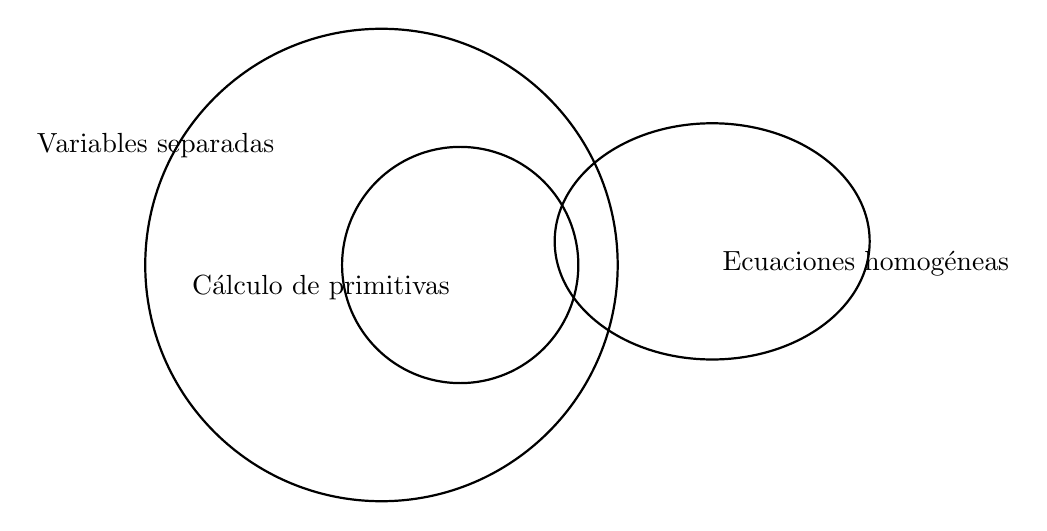
\begin{tikzpicture}
    % Conjunto B
    \draw[thick] (0,0) circle (3cm) node[above left=35pt] {Variables separadas};
    
    % Conjunto A (dentro de B)
    \draw[thick] (1,0) circle (1.5cm) node[below left] {Cálculo de primitivas};
    
    % Conjunto C
    \draw[thick] (4.2,0.3) ellipse (2cm and 1.5cm) node[below right] {Ecuaciones homogéneas};
\end{tikzpicture}

Por tanto, nuestra función será ahora de la forma:
\begin{equation*}
    f(t,x) = h\left(\dfrac{x}{t}\right)
\end{equation*}
Por lo que siempre tendremos que excluir la recta $t=0$. Las ecuaciones nos saldrán en dos sectores, a la izquierda o a la derecha.\\

Supongamos que $J = \left]\alpha, \beta\right[$. Entonces:
\begin{equation*}
    \alpha < \frac{x}{t} < \beta
\end{equation*}
Dado un punto $(t,x)$, $\frac{x}{t}$ es la pendiente de dicho punto. Por tanto, estamos con aquellos puntos del plano con inclinación comprendida entre $\alpha$ y $\beta$. Estaremos trabajando en un sector circular.:

% // TODO: (dibujar rectas con pendiente $\alpha$) y $beta$ y quitar el cero
\begin{figure}[H]
\centering
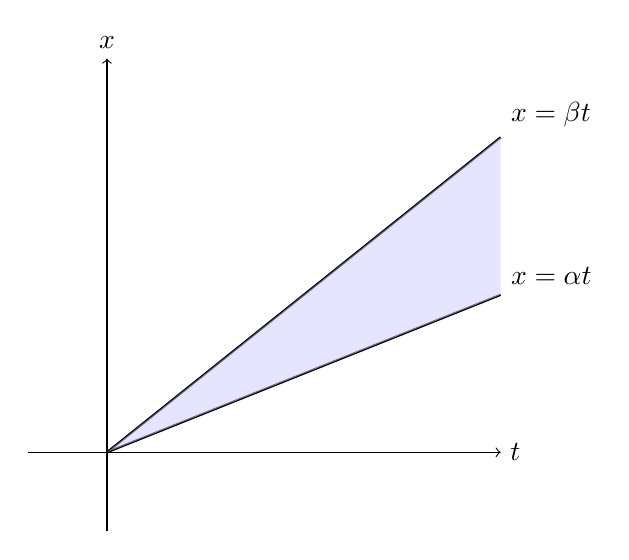
\begin{tikzpicture}
    % Ejes coordenados
    \draw[->] (-1,0) -- (5,0) node[right] {$t$};
    \draw[->] (0,-1) -- (0,5) node[above] {$x$};

    % Recta y = \alpha x
    \draw[thick] (0,0) -- (5,2) node[above right] {$x = \alpha t$};

    % Recta y = \beta x
    \draw[thick] (0,0) -- (5,4) node[above right] {$x = \beta t$};
    
    % Relleno del sector angular entre las rectas
    \fill[blue!20, opacity=0.5] (0,0) -- (5,2) -- (5,4) -- cycle;
\end{tikzpicture}   
\caption{Sector circular, sin incluir el punto $(0,0)$.}
\end{figure}



Por tanto, la ecuación diferencial estará definida en dos dominios posibles (dos sectores angulares):
\begin{gather*}
    D_+ = \left\{(t,x)\in \mathbb{R}^2 \mid t > 0, \dfrac{x}{t}\in J\right\}\\
    D_- = \left\{(t,x)\in \mathbb{R}^2 \mid t < 0, \dfrac{x}{t}\in J\right\}
\end{gather*}
En dichos dominios (ya sea en $D_+$ o $D_-$), la función $f$ será continua:
\begin{equation*}
    (t,x) \mapsto \dfrac{x}{t} \mapsto h\left(\dfrac{x}{t}\right)
\end{equation*}
Ya que las dos funciones que usamos en la composición son continuas.\\

La gracia de estas funciones es que hay un cambio de variable que nos lleva las ecuaciones homogéneas a variables separadas.

El cambio es:
\begin{equation*}
    \varphi : \left\{\begin{array}{rl}
            s &= t \\
            y &= \dfrac{x}{t}
    \end{array}\right.
\end{equation*}
que es fácil comprobar que es un $C^1$-difeomorfismo de clase $C^1(D_+, \mathbb{R}^2)$.
Además, la condición de admisibilidad estará garantizado, ya que no hemos cambiado $t$:
\begin{equation*}
    \dfrac{\partial\varphi_1}{\partial t} + \dfrac{\partial\varphi_1}{\partial x} f = 1 + 0 \neq 0
\end{equation*}

Su cambio inverso será:
\begin{equation*}
    \psi : \left\{\begin{array}{rl}
            t &= s \\
            x &= s y
    \end{array}\right.
\end{equation*}

De esta forma:
\begin{equation*}
    \varphi(D_+) = \left]0, +\infty \right\[ \times J
\end{equation*}

\begin{figure}[H]
\centering
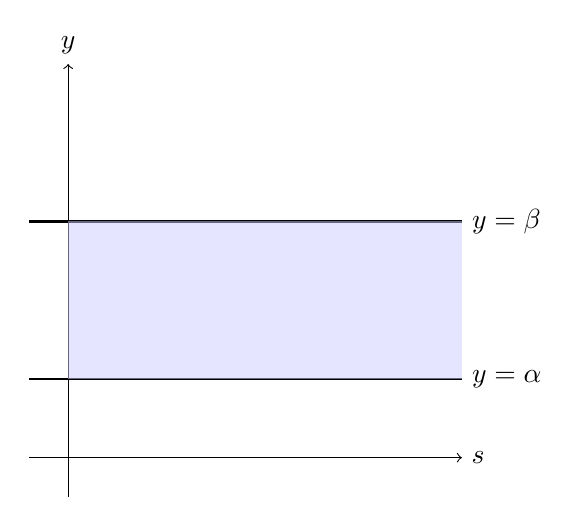
\begin{tikzpicture}
    % Ejes coordenados
    \draw[->] (-0.5,0) -- (5,0) node[right] {$s$}; % Eje x
    \draw[->] (0,-0.5) -- (0,5) node[above] {$y$}; % Eje y

    % Recta y = \alpha
    \draw[thick] (-0.5,1) -- (5,1) node[right] {$y = \alpha$}; % Cambia 1 por el valor que desees para alpha

    % Recta y = \beta
    \draw[thick] (-0.5,3) -- (5,3) node[right] {$y = \beta$};  % Cambia 3 por el valor que desees para beta
    
    % Relleno de la banda entre y = \alpha y y = \beta
    \fill[blue!20, opacity=0.5] (0,1) rectangle (5,3);

\end{tikzpicture}
\caption{Banda horizontal, sin incluir la recta $s = 0$.}
\end{figure}

Ahora, podemos realizar un razonamiento matemático o un cambio formal:\\

De
\begin{equation*}
    \psi : \left\{\begin{array}{rl}
            t &= s \\
            x &= s y
    \end{array}\right.
\end{equation*}

Tenemos que $x = ty$ y pensamos que $x$ e $y$ dependen de $t$:
\begin{equation*}
    \dfrac{dy}{ds} = \dfrac{dy}{dt} \cancelto{1}{\dfrac{dt}{ds}} = 
\end{equation*}

% // TODO: Cambiar por df/ds
\begin{equation*}
    x' = ty' + y
\end{equation*}
\begin{equation*}
    x' = h\left(\dfrac{x}{t}\right) = h(y)
\end{equation*}
Despejamos $y'$ y llegamos a que:
\begin{equation*}
    y' = \dfrac{1}{t} [h(y)-y]
\end{equation*}
Con lo que llegamos a que:
\begin{equation*}
    \dfrac{dy}{ds} = \dfrac{1}{s} [h(y)-y]
\end{equation*}
Que es una ecuación de variables separadas, luego toda ecuación homogénea puede llevarse a una ecuación de variables separadas.\\

Recordamos que en variables separadas había dos soluciones:
\begin{itemize}
    \item Constantes.
    \item No constantes.
\end{itemize}
Y no debemos olvidarnos las soluciones constantes.
Observemos que cuando $h(b)-b=0$, encontramos soluciones constantes de la ecuación diferencial, que serán las funciones:
\begin{equation*}
    z(s) = b
\end{equation*}
Que al deshacer el cambio de variable, nos darán una semirrecta en el dominio original:
\begin{equation*}
    x(t) = b\cdot t
\end{equation*}

% // TODO: Definir problema de valores iniciales, PVI
\begin{ejemplo}
    Dada la ecuación diferencial (en la que usamos la notación geométrica en lugar de la física):
    \begin{equation*}
        y' = \dfrac{y-x}{y+x}
    \end{equation*}
    Nos disponemos a encontrar una solución de dicha ecuación, cogiendo como condición:
    \begin{equation*}
        y(-1) = -1
    \end{equation*}
    Es una ecuación homogénea, ya que se trata de un cociente de dos polinomios homogéneos de grado 1. Podemos comprobarlo dividiendo numerador y denominador entre $x$.

    La función $h$ a escoger sería:
    \begin{equation*}
        h(\xi) = \dfrac{\xi - 1}{\xi + 1}
    \end{equation*}
    Por lo que el dominio de definición será: $J_- = \left]-\infty, -1\right[$ o $J_+ = \left]-1, +\infty\right[$.\\
    Como queremos que $y(-1) = -1$, buscamos tener $\dfrac{y}{x} = 1$, luego tomaremos $J = J_+$, ya que contiene el 1.
    % // TODO: No sé por qué cogemos este dominio, pero nos quedamos con:
    \begin{equation*}
        D = \left\{(x,y)\in \mathbb{R}^2 \mid x<0, \dfrac{y}{x}>-1\right\}
    \end{equation*}
    Cojemos $x<0$ ya que estamos interesados que el punto $-1$ esté en el dominio de $y$.

    Ahora, haremos el cambio de variable, con variables $u$ y $v$:
    \begin{equation*}
        \left\{\begin{array}{rl}
                u &= x \\
                v &= \dfrac{y}{x}
        \end{array}\right.
    \end{equation*}
    Tratamos de ver ahora qué conjunto manejamos en el codominio:

    % // TODO: COger x < 0
\begin{figure}[H]
\centering
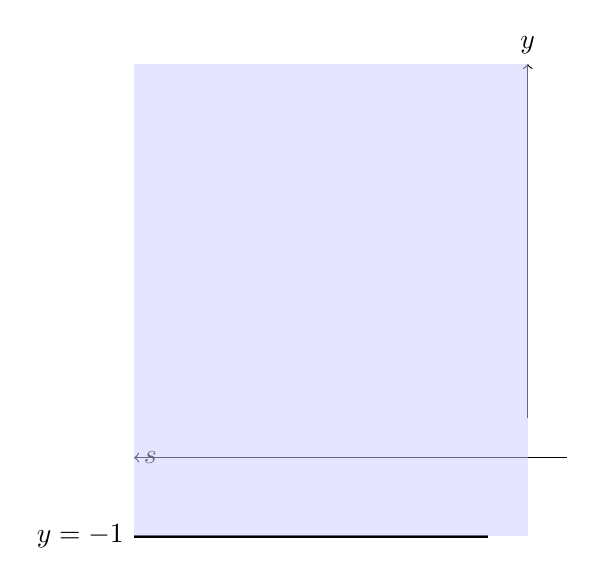
\begin{tikzpicture}
    % Ejes coordenados
    \draw[->] (0.5,0) -- (-5,0) node[right] {$s$}; % Eje x
    \draw[->] (0,0.5) -- (0,5) node[above] {$y$}; % Eje y

    % Recta y = \alpha
    \draw[thick] (-0.5,-1) -- (-5,-1) node[left] {$y = -1$}; % Cambia 1 por el valor que desees para alpha
    
    % Relleno de la banda entre y = \alpha y y = \beta
    \fill[blue!20, opacity=0.5] (0,-1) rectangle (-5,5);

\end{tikzpicture}
\caption{Dominio tras hacer el cambio de variable}
\end{figure}

 Y el punto de la solución, $(-1,-1)$ pasa al punto $(-1,1)$.

 \begin{equation*}
     y = xv
 \end{equation*}

 \begin{equation*}
     y' = v + xv'
 \end{equation*}
 \begin{equation*}
     y' = \dfrac{y-x}{y+x} = \dfrac{\dfrac{y}{x}-1}{\dfrac{y}{x}+1} = \dfrac{v-1}{v+1}
 \end{equation*}
 Nos queda:
 \begin{equation*}
     x\dfrac{dv}{dx} = \dfrac{v-1}{v+1} - v = \dfrac{v-1}{v+1} -\dfrac{v^2 + v}{v+1}
 \end{equation*}

 \begin{equation*}
     \dfrac{dv}{dx} = \dfrac{-1}{x}\cdot \dfrac{1+v^2}{1+v}
 \end{equation*}
 Tenemos nuestra ecuación de variables separadas, que pasamos a resolver. Lo primero a observar es que nos interesa la solución concreta $v$ tal que $v(-1)=1$.\\

 Observamos que la ecuación anterior no tienen soluciones constantes, por ser:
 \begin{equation*}
     \dfrac{1+v^2}{1+v} > 0
 \end{equation*}
 Luego resolvemos por variables separadas:
 \begin{equation*}
     \int \dfrac{1+v}{1+v^2}~dv = -\int \dfrac{dx}{x}
 \end{equation*}
 \begin{equation*}
     -\int \dfrac{dx}{x}= -\ln(-x) + k
 \end{equation*}
 Y la primera integral la partimos en dos para resolverla:
 \begin{equation*}
     \int \dfrac{1+v}{1+v^2}~dv = \arctg v +\dfrac{1}{2}\ln(1+v^2)
 \end{equation*}
 Por tanto:
 \begin{equation*}
     \arctg v + \dfrac{1}{2}\ln(1+v^2) = -\ln(-x) + k
 \end{equation*}
 Que sabemos que va a tener soluciones que definen funciones (lo vimos teóricamente) $v$ en función de $x$.\\

 Ahora, volveremos al dominio original:
 \begin{equation*}
     \arctg\left(\dfrac{y}{x}\right) + \dfrac{1}{2}\ln\left(1+\dfrac{y^2}{x^2}\right) = -\ln(-x) + k
 \end{equation*}
 Que define $y$ como función de $x$ de forma implícita.

 Usando que:
 \begin{equation*}
     \ln(-x) = \dfrac{1}{2}\ln(x^2)
 \end{equation*}

 Despejamos y:
 \begin{equation*}
     \arctg\left(\dfrac{y}{x}\right) + \ln\left(\sqrt{x^2+y^2}\right) = k
 \end{equation*}
Es la familia de soluciones que nos resuelven la ecuación diferencial. Buscamos $k$ para $y(-1)=-1$, sustituyendo $y$ y $x$ por $-1$:
\begin{equation*}
    k = \dfrac{\pi}{4} + \ln\left(\sqrt{2}\right)
\end{equation*}
Para ver que esto define una ecuación implícita, deberíamos aplicar el Teorema, pero gracias a la teoría que venimos desarrollando hasta ahora, lo tenemos visto.
Tenemos visto que dicha fórmula dos define una ecuación implícita en un entorno del punto $(-1,-1)$.

Sin embargo, es un problema específico en el que podemos llegar a ver algo más.
Se trata de una curva que en cartesianas tiene una expresión endiablada, pero en coordenadas polares se ve de una forma muy fácil:

\begin{gather*}
    x = r\cos \theta \\
    y = r\sen \theta
\end{gather*}
\begin{equation*}
    \dfrac{y}{x} = \tan \theta
\end{equation*}
\begin{equation*}
    \arctg(\tg \theta)
\end{equation*}
No es siempre igual a $\theta$, sólo en $\left]-\frac{\pi}{2}, \frac{\pi}{2}\right[$.
Como estamos en el 3er cuadrante: $\theta \in \left]\frac{\pi}{2}, \frac{3\pi}{2}\right[$:
\begin{equation*}
    \arctg(\tg \theta) = \arctg(\tg(\theta - \pi)) = \theta - \pi
\end{equation*}
donde se usa que la $\tg$ es $\pi$-periódica.

\begin{equation*}
    \theta + \ln r = k + \pi
\end{equation*}
Se trata de la espiral logarítmica o de Arquímedes, que se entiende mejor tomando:
\begin{equation*}
    r = e^{k-\theta+\pi}
\end{equation*}
Fijado un $r$, conforme movemos $\theta$, se va formando una especie de circunferencia pero con $r$ disminuyendo, luego se forma una espiral.

Notemos que las espirales son curvas de la forma
\begin{equation*}
    r = f(\theta)
\end{equation*}
con $f$ creciente y decreciente.
\end{ejemplo}

\subsection{Ecuaciones reducibles a homogéneas}
Son como las ecuaciones homogéneas salvo por que tienen un polinomio de primer grado en el numerador y denominador:
\begin{equation*}
    x' = h\left(\dfrac{at + bx + c}{At + Bx + C}\right) \qquad a,b,c,A,B,C \in \mathbb{R}
\end{equation*}
Con $h:I\rightarrow\mathbb{R}$ una función continua con $I$ un intervalo abierto.

\begin{ejercicio}
    Determinar cuál sería el dominio de la ecuación diferencial superior.
\end{ejercicio}

El truco que funciona casi siempre es realizar una traslación:\\

Defino:
\begin{equation*}
    \left\{\begin{array}{rl}
            s &= t - t_* \\
            y &= x - x_*
    \end{array}\right. \qquad (t_*, x_*)\in \mathbb{R}^2
\end{equation*}
% // TODO: Ver que es un cambio admisible

El cambio de variable es:
% // TODO: Hacer con rigor
\begin{equation*}
    \dfrac{dy}{ds} = \dfrac{dx}{dt} = f(t,x)
\end{equation*}

Y hay que quitar las variables $t$ y $x$:
\begin{equation*}
    \dfrac{dy}{ds} = h\left(\dfrac{a(s+t_*)+b(y+x_*)+c}{A(s+t_*)+B(y+x_*)+C}\right)
\end{equation*}

Y si conseguimos hacer :
\begin{gather*}
    xt_* + bx_* + c = 0 \\
    At_* + Bx_* + C = 0
\end{gather*}
Nos quedaría que:
\begin{equation*}
    \dfrac{dy}{ds} = h\left(\dfrac{a(s+t_*)+b(y+x_*)+c}{A(s+t_*)+B(y+x_*)+C}\right) = h\left(\dfrac{as + by}{As+By}\right)
\end{equation*}
Que se trata de una ecuación homogénea.\\

Las reducidas a homogéneas se pasan a homogéneas de forma que el punto $(t_*, x_*)$ sean solución del sistema anterior. No tenemos garantía de que esto pase, ya que el sistema ha de tener soluciones (el determinante distinto de 0).\\

Nos queda un caso que no está cubierto, el caso en el que dicho sistema es incompatible. En dicho caso, entonces:
\begin{equation*}
    det(ab AB) = 0
\end{equation*}
Por tanto, los vectores $(a,b)$ y $(A,B)$ son linealmente dependientes en $\mathbb{R}^2$, luego podremos poner uno en función del otro. Suponemos que podemos hacer (si no, el otro):
\begin{equation*}
    (A,B) = \lm(a,b)\qquad \lm \in \mathbb{R}
\end{equation*}
Sustituimos y:
\begin{equation*}
    x' = h\left(\dfrac{at + bx +c}{\lm(at+bx)+C}\right)
\end{equation*}
Que no es una ecuación homogénea pero nos permite hacer el cambio de variable (suponiendo que $b\neq 0$):
\begin{equation*}
    at + bx &= y \\
\end{equation*}

\begin{ejemplo}
    Un problema que podemos encontrarnos es:
    \begin{equation*}
        x' = \dfrac{x+t+1}{x-t+3}\qquad x(0)=0
    \end{equation*}
    Encuentre la solución a este problema y diga en qué intervalo está definido.
\end{ejemplo}
